\documentclass[UTF8]{ctexart}

% PACKAGES FOR TITLES
\usepackage{titlesec}
\usepackage{color}

\usepackage{graphicx}
\graphicspath{ {../../../rc/} }

\usepackage{minted}

\usepackage{subfig} % Numbered and caption subfigures using \subfloat
\usepackage{caption} % Coloured captions
\usepackage{transparent}

% STANDARD MATH PACKAGES
\usepackage{amsmath}
\usepackage{amsthm}
\usepackage{bm}
\usepackage[overload]{empheq}  % For braced-style systems of equations

% PACKAGES FOR TABLES
\usepackage{array}
\usepackage{tabularx}
\usepackage{longtable} % tables that can span several pages
\usepackage{colortbl}

% PACKAGES FOR ALGORITHMS (PSEUDO-CODE)
\usepackage{algorithm}
\usepackage{algorithmic}

% PACKAGES FOR ITEMIZE & ENUMERATES 
\usepackage{enumitem}

% PACKAGES FOR REFERENCES & BIBLIOGRAPHY
\usepackage[colorlinks=true,linkcolor=black,anchorcolor=black,citecolor=black,filecolor=black,menucolor=black,runcolor=black,urlcolor=black]{hyperref} % Adds clickable links at references

\usepackage{url}
\usepackage{hyperref}
\usepackage{cleveref}
\usepackage[square, numbers, sort&compress]{natbib} % Square brackets, citing references with numbers, citations sorted by appearance in the text and compressed
\bibliographystyle{plain} % You may use a different style adapted to your field

% OTHER PACKAGES
\usepackage{amsthm,thmtools,xcolor} % Coloured "Theorem"
\usepackage{comment} % Comment part of code
\usepackage{fancyhdr} % Fancy headers and footers
\usepackage{lipsum} % Insert dummy text
\usepackage{tcolorbox} % Create coloured boxes (e.g. the one for the key-words)

% Do not change Configuration_files/config.tex file unless you really know what you are doing. 
% This file ends the configuration procedures (e.g. customizing commands, definition of new commands)
% Configuration package
\usepackage[bottom=2.0cm,top=2.0cm,left=2.0cm,right=2.0cm]{geometry}


% Create color bluePoli (-> manuale grafica coordinata:  https://www.polimi.it/fileadmin/user_upload/il_Politecnico/grafica-coordinata/2015_05_11_46xy_manuale_grafica_coordinata.pdf)
\definecolor{bluePoli}{cmyk}{0.4,0.1,0,0.4}

% Custom theorem environments
\declaretheoremstyle[
  headfont=\color{bluePoli}\normalfont\bfseries,
  bodyfont=\color{black}\normalfont\itshape,
]{colored}

\captionsetup[figure]{labelfont={color=bluePoli}} % Set colour of the captions
\captionsetup[table]{labelfont={color=bluePoli}} % Set colour of the captions
\captionsetup[algorithm]{labelfont={color=bluePoli}} % Set colour of the captions

\theoremstyle{colored}
\newtheorem{theorem}{Theorem}[section]
\newtheorem{proposition}{Proposition}[section]

% Enhances the features of the standard "table" and "tabular" environments.
\newcommand\T{\rule{0pt}{2.6ex}}
\newcommand\B{\rule[-1.2ex]{0pt}{0pt}}

% Algorithm description
\newcounter{algsubstate}
\renewcommand{\thealgsubstate}{\alph{algsubstate}}
\newenvironment{algsubstates}{
    \setcounter{algsubstate}{0}%
    \renewcommand{\STATE}{%
    \stepcounter{algsubstate}%
    \Statex {\small\thealgsubstate:}\space}
    }{}
    
% Custom theorem environment
%\newcolumntype{L}[1]{>{\raggedright\let\newline\\\arraybackslash\hspace{0pt}}m{#1}}
\newcolumntype{C}[1]{>{\centering\let\newline\\\arraybackslash\hspace{0pt}}m{#1}}
%\newcolumntype{R}[1]{>{\raggedleft\let\newline\\\arraybackslash\hspace{0pt}}m{#1}}

% Custom itemize environment
\setlist[itemize,1]{label=$\bullet$}
\setlist[itemize,2]{label=$\circ$}
\setlist[itemize,3]{label=$-$}
\setlist{nosep}

% Create command for background pic
\newcommand\BackgroundPic{% Adding background picture
	\put(237,365){
	    \parbox[b][\paperheight]{\paperwidth}{%
	    \vfill
		\centering
		\transparent{0.4}
		%\includegraphics[width=0.44\paperwidth]{raggiera_polimi.eps}%
		\vfill}
		}
}

% Set indentation
\setlength\parindent{0pt}

% Custom title commands
\titleformat{\section}
{\color{bluePoli}\normalfont\Large\bfseries}
{\color{bluePoli}\thesection.}{1em}{}
\titlespacing*{\section}
{0pt}{3.3ex}{3.3ex}

\titleformat{\subsection}
{\color{bluePoli}\normalfont\large\bfseries}
{\color{bluePoli}\thesubsection.}{1em}{}
\titlespacing*{\subsection}
{0pt}{3.3ex}{3.3ex}

% Custom headers and footers
\pagestyle{fancy}
\fancyhf{}
      
\fancyfoot{}
\fancyfoot[C]{\thepage} % page
\renewcommand{\headrulewidth}{0mm} % headrule width
\renewcommand{\footrulewidth}{0mm} % footrule width

\makeatletter
\patchcmd{\headrule}{\hrule}{\color{black}\hrule}{}{} % headrule
\patchcmd{\footrule}{\hrule}{\color{black}\hrule}{}{} % footrule
\makeatother


\title{Deep Into Graphics Rendering}
\author{wegatron}
\date{2021.11.2}

\begin{document}
\CJKfamily{zhkai}
\maketitle

\begin{abstract}
	本文介绍图形渲染相关的一些重要的基础知识. 在“拥抱现代图形API”, 首先通过现代和传统图形API的对比, 阐述了现代图形API的优势. 然后, 分析了使用现代图形API开发的一些挑战, 并给出了基于现代图形API的渲染管线设计的一些常规的思路. 其后, 在“深入理解GPU硬件运行机制”一章中, 以Nvidia显卡为例, 介绍了GPU的硬件设计, 以及渲染工作在GPU中的执行过程. 在该章末尾, 着重介绍了GPU中的几个重要技术. 最后一章简单介绍了一些渲染优化的简单建议.
\end{abstract}

\section{拥抱现代图形API}
参考《游戏引擎随笔0x05: 现代图形API讲义》\cite{modernGraphicsAPI}
\subsection{现代图形API VS 传统图形API}
传统图形API: OpenGL(ES), D3D\\
现代图形API: Vulkan, Metal, D3D12\\
比喻:
\begin{itemize}
\item 公交车(传统图形API-固定管线), 满足大众常用的出行需求, 无法定制且出行效率低. 使用代价最低(廉价).
\item 打车(传统图形API-可编程管线), 可以自定义出行起点+终点(甚至可以提出一些路线或速度上的要求), 但任然需要一定的等待, 但最终得依靠司机, 无法满足一些特殊的需求(如在偏僻地方打不上车). 使用代价增高.
\item 自驾车(现代图形API), 完全掌控自己的出行路线、时间、速度等. 使用代价最高(需要自己会开).
  \begin{itemize}
  \item 自动档(Metal), 做了部分自动化, 使用方便且不失性能.
  \item 手动档(Vulkan), 暴露了很多细节, 使用难度更大, 可操控性更强.
  \end{itemize}
\item 辅助驾驶(UE等渲染引擎), 结构复杂, 自动化程度高.
\end{itemize}

现代图形API与传统图形API要点比较:

\begin{itemize}
\item 渲染管线状态维护
  \\传统的图形API使用隐式、全局的状态管理机制. 缺陷: 1.无法精准的控制管线当前状态; 2.应用程序必须频繁的调用API来设置管线状态和恢复; 3.API还会对每个渲染状态的设置进行校验和二次处理, 比如合并状态统一提交(新型 GPU 会将这些固定管线状态合并成单一硬件状态, 因此需要Driver在运行时为不同的状态组合创建、查找缓存内部的管线状态集合, 这很可能会导致管线卡顿, 同时额外增大了开销).
  \begin{figure}[H]
    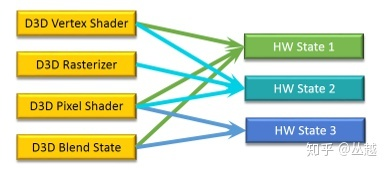
\includegraphics[width=10cm]{render_state_merge.jpg}
    \centering
    \caption{D3D11分散的状态对象设置导致图形硬件切换的额外开销}
    \label{fig:gpu_rendering_pipline_state_merge}
  \end{figure}

  现代图形API使用PipelineState将管道状态提前创建并绑定, 在渲染时, 通过设置不同的 PipelineState, Driver只需要少量的切换开销即可将预先创建的状态绑定到GPU中, 而无需像传统API那样校验每种状态有效性以及动态合并状态, 从而降低了绘制调用开销, 并且可以大幅增加每帧的绘制调用次数.

  \begin{figure}[H]
    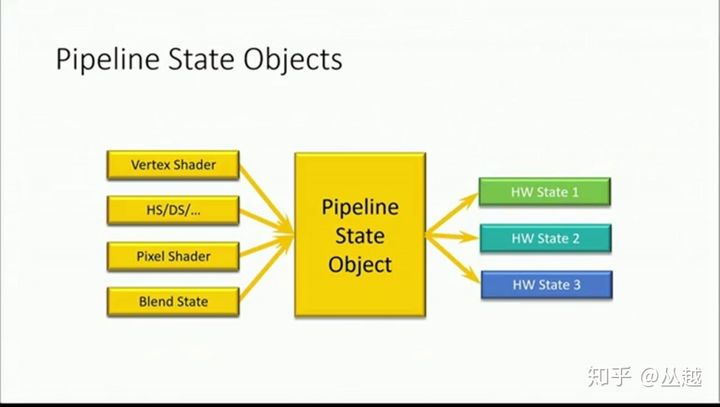
\includegraphics[width=10cm]{pipline_state_object.jpg}
    \centering
    \caption{PipelineState 将管道状态提前创建并绑定}
    \label{fig:graphics_pipeline_state}
  \end{figure}
\item 资源绑定
  \\与渲染管线状态类似, 传统图形API逐个API调用来实现资源的绑定. 而现代图形API通过RootSingature(D3D12) 或者PipelineLayout(Vulkan) 通过Descriptor预先设置好Shader所需要使用的资源布局信息, 包括:Constant、Texture(SRV)、Buffer(UAV)、Sampler 等, 在渲染时Shader通过DescriptorTable或者DescriptorSet用间接寻址方式获取资源, 无需渲染时绑定, 大大降低了资源绑定和校验开销, 从而提高了渲染性能.
  \\Metal 虽然也有 PipelineState, 但并没有提供指定 Shader Resource Layout的机制.
  \begin{figure}[H]
    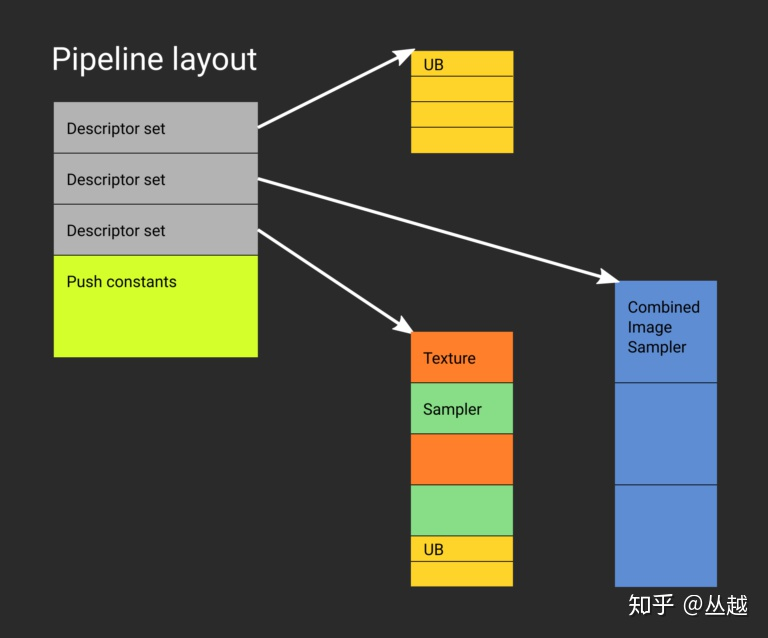
\includegraphics[width=10cm]{data_resource_binding.jpg}
    \centering
    \caption{Vulkan的Pipeline Layout使用DescriptorSet间接引用Shader资源}
    \label{fig:data_resource_binding}
  \end{figure}
\item 显式内存管理
  \\传统的API的内存管理是隐式的, 当创建资源时 Runtime/Driver 内部也同时创建用于这个资源的内存, 这个过程对开发者是透明的, 尽管接口简单, 但带来的问题是很难优化内存分配, 并且容易造成 GPU 内存碎片.
  \\现代API 都提供了 CPU/GPU 堆内存管理接口, 可以通过创建堆, 在堆上分配空间的方式来创建资源, 应用程序可以精准的控制资源堆内存的分配. 比如可以通过资源别名(在同一堆空间中创建不同的资源), 在不同的时段可重复利用同一的设备内存来完成渲染逻辑, 从而更有效的使用有限的 GPU 内存资源.
  \begin{figure}[H]
    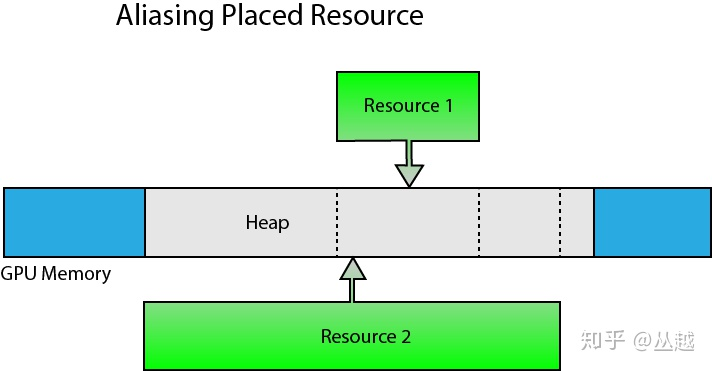
\includegraphics[width=10cm]{gpu_aliasing_placed_resource.jpg}
    \centering
    \caption{在重叠的GPU堆空间中创建不同的资源}
    \label{fig:aliasing_placed_resource}
  \end{figure}
\item 状态的跟踪和同步
  \\传统 API 在 Driver 内部维护跟踪状态, 自动管理资源及调度, 以及进行运行时的校验. Driver 还要负责 CPU 与 GPU 的同步. 典型的例子: 动态更新 GPU Buffer 数据, 如果此时 GPU 正在使用这个 Buffer, 则 Map/Lock 之后 API返回的是 Runtime/Driver 内部动态创建的新内存地址, 以更新新数据, 当 GPU 使用完旧内存后, 再使用新数据. 另外, API 的提示标记并不能保证 Driver 一定按照预想的方式执行, Driver 会根据自身当前的状态来决定, 比如上述情况, 即使在 Map 时指定了 Discard, 也不能完全保证运行时 CPU 和 GPU 是完全异步的.
  \\现代 API 通过使用资源屏障 (Resource Barrier) 来要求应用层明确控制资源的状态迁移, 通过Fence对象和WaitFence函数完成CPU和GPU的同步. 整个过程完全由应用程序来控制, 这样应用程序可以根据需要, 更加精准的控制同步时机.
\item 并行渲染
  \\现代 API 都增加了 Command List 或 Command Buffer 记录渲染指令, 再通过 Queue 提交到 GPU 中, 而每个 Command List/Buffer 都可以在不同的线程中单独填充, 这意味着可以并行录制渲染指令, 充分发挥了现代 CPU 多核的并行能力. 甚至还可以创建多个异步计算或者上传数据的 Command Queue, 利  用 GPU 的并行机制实现渲染和计算、上传数据的并行.
\item shader code
  \\Shader Code预编译机制
\item 附加模块支持
  \begin{itemize}
  \item RayTracying
  \item ML: Vulkan ML, Metal Performance Shader
  \end{itemize}
\end{itemize}

\subsection{基于现代图形 API 开发的挑战}
要在现代 API 基础上实现更好的性能, 需要更多更复杂的图形管线管理开发工作. 由于是显式的, 更接近图形硬件的设计, 现代 API 的驱动不再负责传统 API Driver 复杂的内部逻辑, 但这些工作并不是自动消失, 而是转移到应用层, 由开发者负责. 传统 API 上和现代 API 上图形管线管理开发工作量的比较:
\begin{figure}[H]
  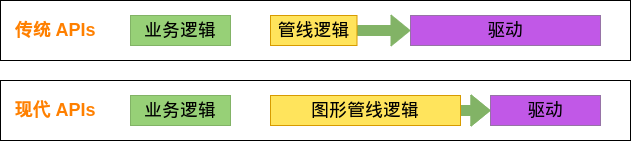
\includegraphics[width=10cm]{graphics_works.png}
  \centering
  \caption{基于传统API和现代API上图形管线管理代码量的比较}
  \label{fig:works_comparation}
\end{figure}

这些工作量包括:
\begin{itemize}
\item 重新设计图形 API 抽象接口.
  \\通过PipelineState对象来维护渲染管线状态, Command List录制图形指令, 实现并行渲染. 资源屏障等, 来进行同步.

\item 堆内存管理.
  \\包括 GPU 和 CPU 内存, 精细控制内存预算和跟踪内存分配和使用, 甚至还要根据不同使用场景来定制内存管理策略. 比如根据 GPU 是否只读、CPU 是否只读、CPU/GPU 的写入频率等, 不同的情况需要对应不同的内存管理策略, 充分利用 GPU 的 Copy/Upload/Transfer 硬件引擎完成数据传输, 才能实现最佳的性能.

\item 描述符(Descriptor)管理
  \\在传统 API 上绑定 Shader 资源只需要简单调用形如 SetTexture/SetConstant/SetSampler 之类的接口即可, 而在现代 API 中, 通过 Shader 所需要使用的资源布局信息是预置的(前文所述), 渲染时需要通过 Descriptor 来间接寻址资源, 由于 Descriptor 也是一种 API(GPU 硬件) 资源, 一般来说 GPU 可见的 Descriptor 是有限的(硬件相关限制), 渲染时需要对有限的 GPU Descriptor 使用有效的管理方式加以重用, 才能完成复杂的渲染逻辑. 另外由于并行渲染的存在, Descriptor 的分配和释放还要考虑到线程同步, 如何在并行中减少线程同步所带来的开销也是需要仔细考虑的问题, 这进一步增加了管理复杂度.

\item 渲染帧管理
  \\为了最大化并行 CPU/GPU, Swapchain 通常需要创建多个back Buffer, 这样 GPU 绘制当前帧(或者上一帧), CPU 可以并行填充绘制下一帧的命令, 在开始录制每个 Frame 的渲染指令时, 可以通过这一帧上一次绘制的 GPU Fence 查询 GPU 是否完成上一次渲染, 如果完成则开始录制逻辑, 否则等待. 要达到这样的结果, 每个 Frame 需要有自己的 CommandList 和相关的 GPU 资源, 这就需要实现渲染帧逻辑, 还需要在提交到 GPU 渲染时对 Frame 进行调度管理.
  \begin{figure}[H]
    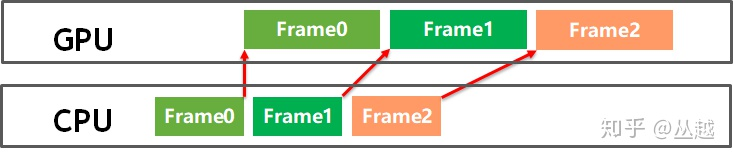
\includegraphics[width=10cm]{frame_management.jpg}
    \centering
    \caption{并行渲染}
    \label{fig:parallel_rendering}
  \end{figure}

\item API 对象的生命周期控制
  \\要保证 API 渲染、计算管线中在使用对象的过程中不能释放对象. 比如上层逻辑在 Frame2 中释放某个对象, 但这个对象还在 Frame1 中被使用, 则此时不能执行真正的释放, 需要通过 GPU Fence 事件通知或者轮询方式等到 Frame1 执行完成才能释放.

\item 并行提交绘制指令
  \\现代 API 的 Command List 都是 Thread Free 的, 所以可以实现多个线程并行填充绘制、计算指令, 以达到并行提交渲染工作的的目的. 可利用Task/Job System来实现.
\end{itemize}

\subsection{基于现代图形 API 的渲染管线设计}
GPU 并行架构
利用并行提交特性, 渲染管线可设计为多线程结构, 可根据当前 CPU 硬件线程数量动态决定 CommandList/Buffer 的数量, 这样在架构上也是可缩放的。

另外, 现代GPU其内部都会有多个专用于不同功能的GPU硬件, 一般可以抽象为图形(3D)、计算(Compute)、Copy(Transfer)三种, 这三者在 GPU 内部可并行执行, 如下图所示:

\begin{figure}[H]
  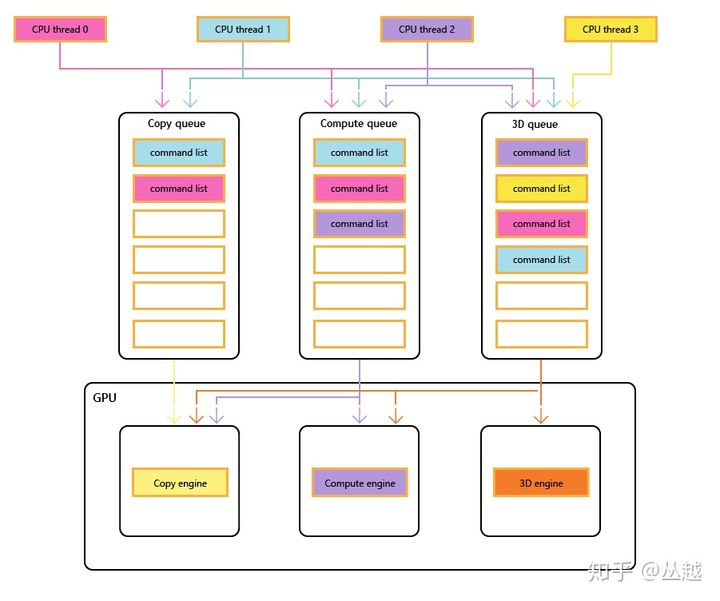
\includegraphics[width=10cm]{rendering_framework.jpg}
  \centering
  \caption{GPU硬件功能抽象}
  \label{fig:gpu_hardware_abstraction}
\end{figure}

利用这个机制可以将管线设计为这样:
\begin{figure}[H]
  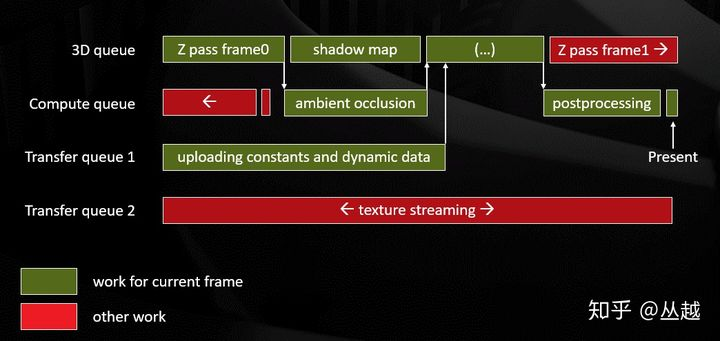
\includegraphics[width=10cm]{rendering_pipeline_design.jpg}
  \centering
  \caption{GPU渲染管线的初步设计}
  \label{fig:gpu_rendering_pipeline_design_0}
\end{figure}

如图所示, 图形(3D)队列负责 PreZ、GBuffer、Shadow 等场景渲染, 同时计算队列负责计算后处理(SSAO、Bloom、ToneMapping、AA 等等), Copy 队列同时执行纹理 Streaming 或者 Virtual texture 等操作。这些都可以在 GPU 时间线上同时进行, 大大提高了渲染管线的性能.

进一步优化 Render Graph:
通过检查渲染帧内的资源依赖关系, 利用别名资源重复利用内存堆, 优化 GPU 内存资源使用。如下所示:

\begin{figure}[H]
  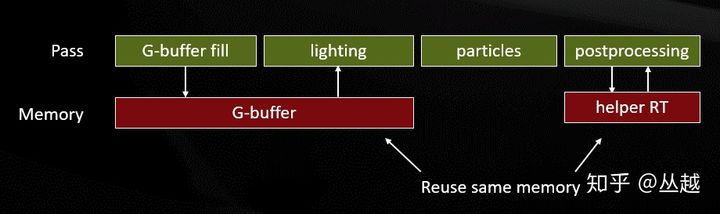
\includegraphics[width=10cm]{rendering_pipeline_design_opt.jpg}
  \centering
  \caption{GPU渲染管线进一步优化}
  \label{fig:gpu_rendering_pipeline_optimization}
\end{figure}

GPU驱动的渲染管线
利用间接绘制/计算(IndirectDraw/IndirectCompute), 可实现渲染时更少的CPU/GPU之间的切换, 在CPU中准备场景数据, 一次性提交到GPU中, 使用GPU进行可见性剔除, 并填充CommandList/Buffer, 这样可以将传统的CPU负担的工作交由GPU执行, 降低CPU的负载, 甚至可以进行更高精度级别的可见性剔除.
\begin{figure}[H]
  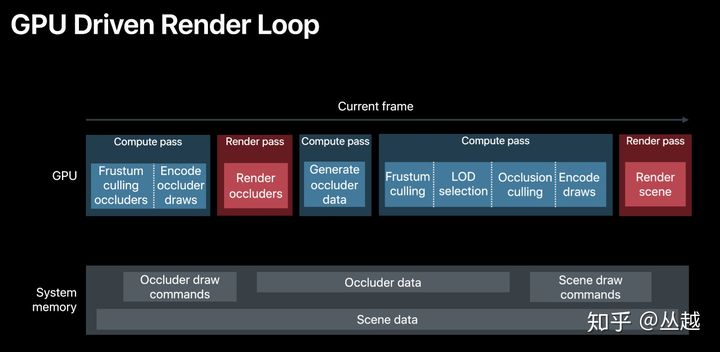
\includegraphics[width=10cm]{gpu_driven_rendering.jpg}
  \centering
  \caption{基于Metal API的GPU驱动渲染管线设计}
  \label{fig:gpu_driven_rendering}
\end{figure}

\section{深入GPU硬件运行机制}
参考《深入GPU硬件架构及运行机制》\cite{deepIntoGPU}
\subsection{了解GPU的硬件}
\subsubsection{GPU中的一些基本概念}
这里以Nvidia Turing架构为例, Turing架构是Nvidia在2018年发布的GPU架构, 其下2060、2080系列显卡均使用该种架构.
\begin{figure}[H]
  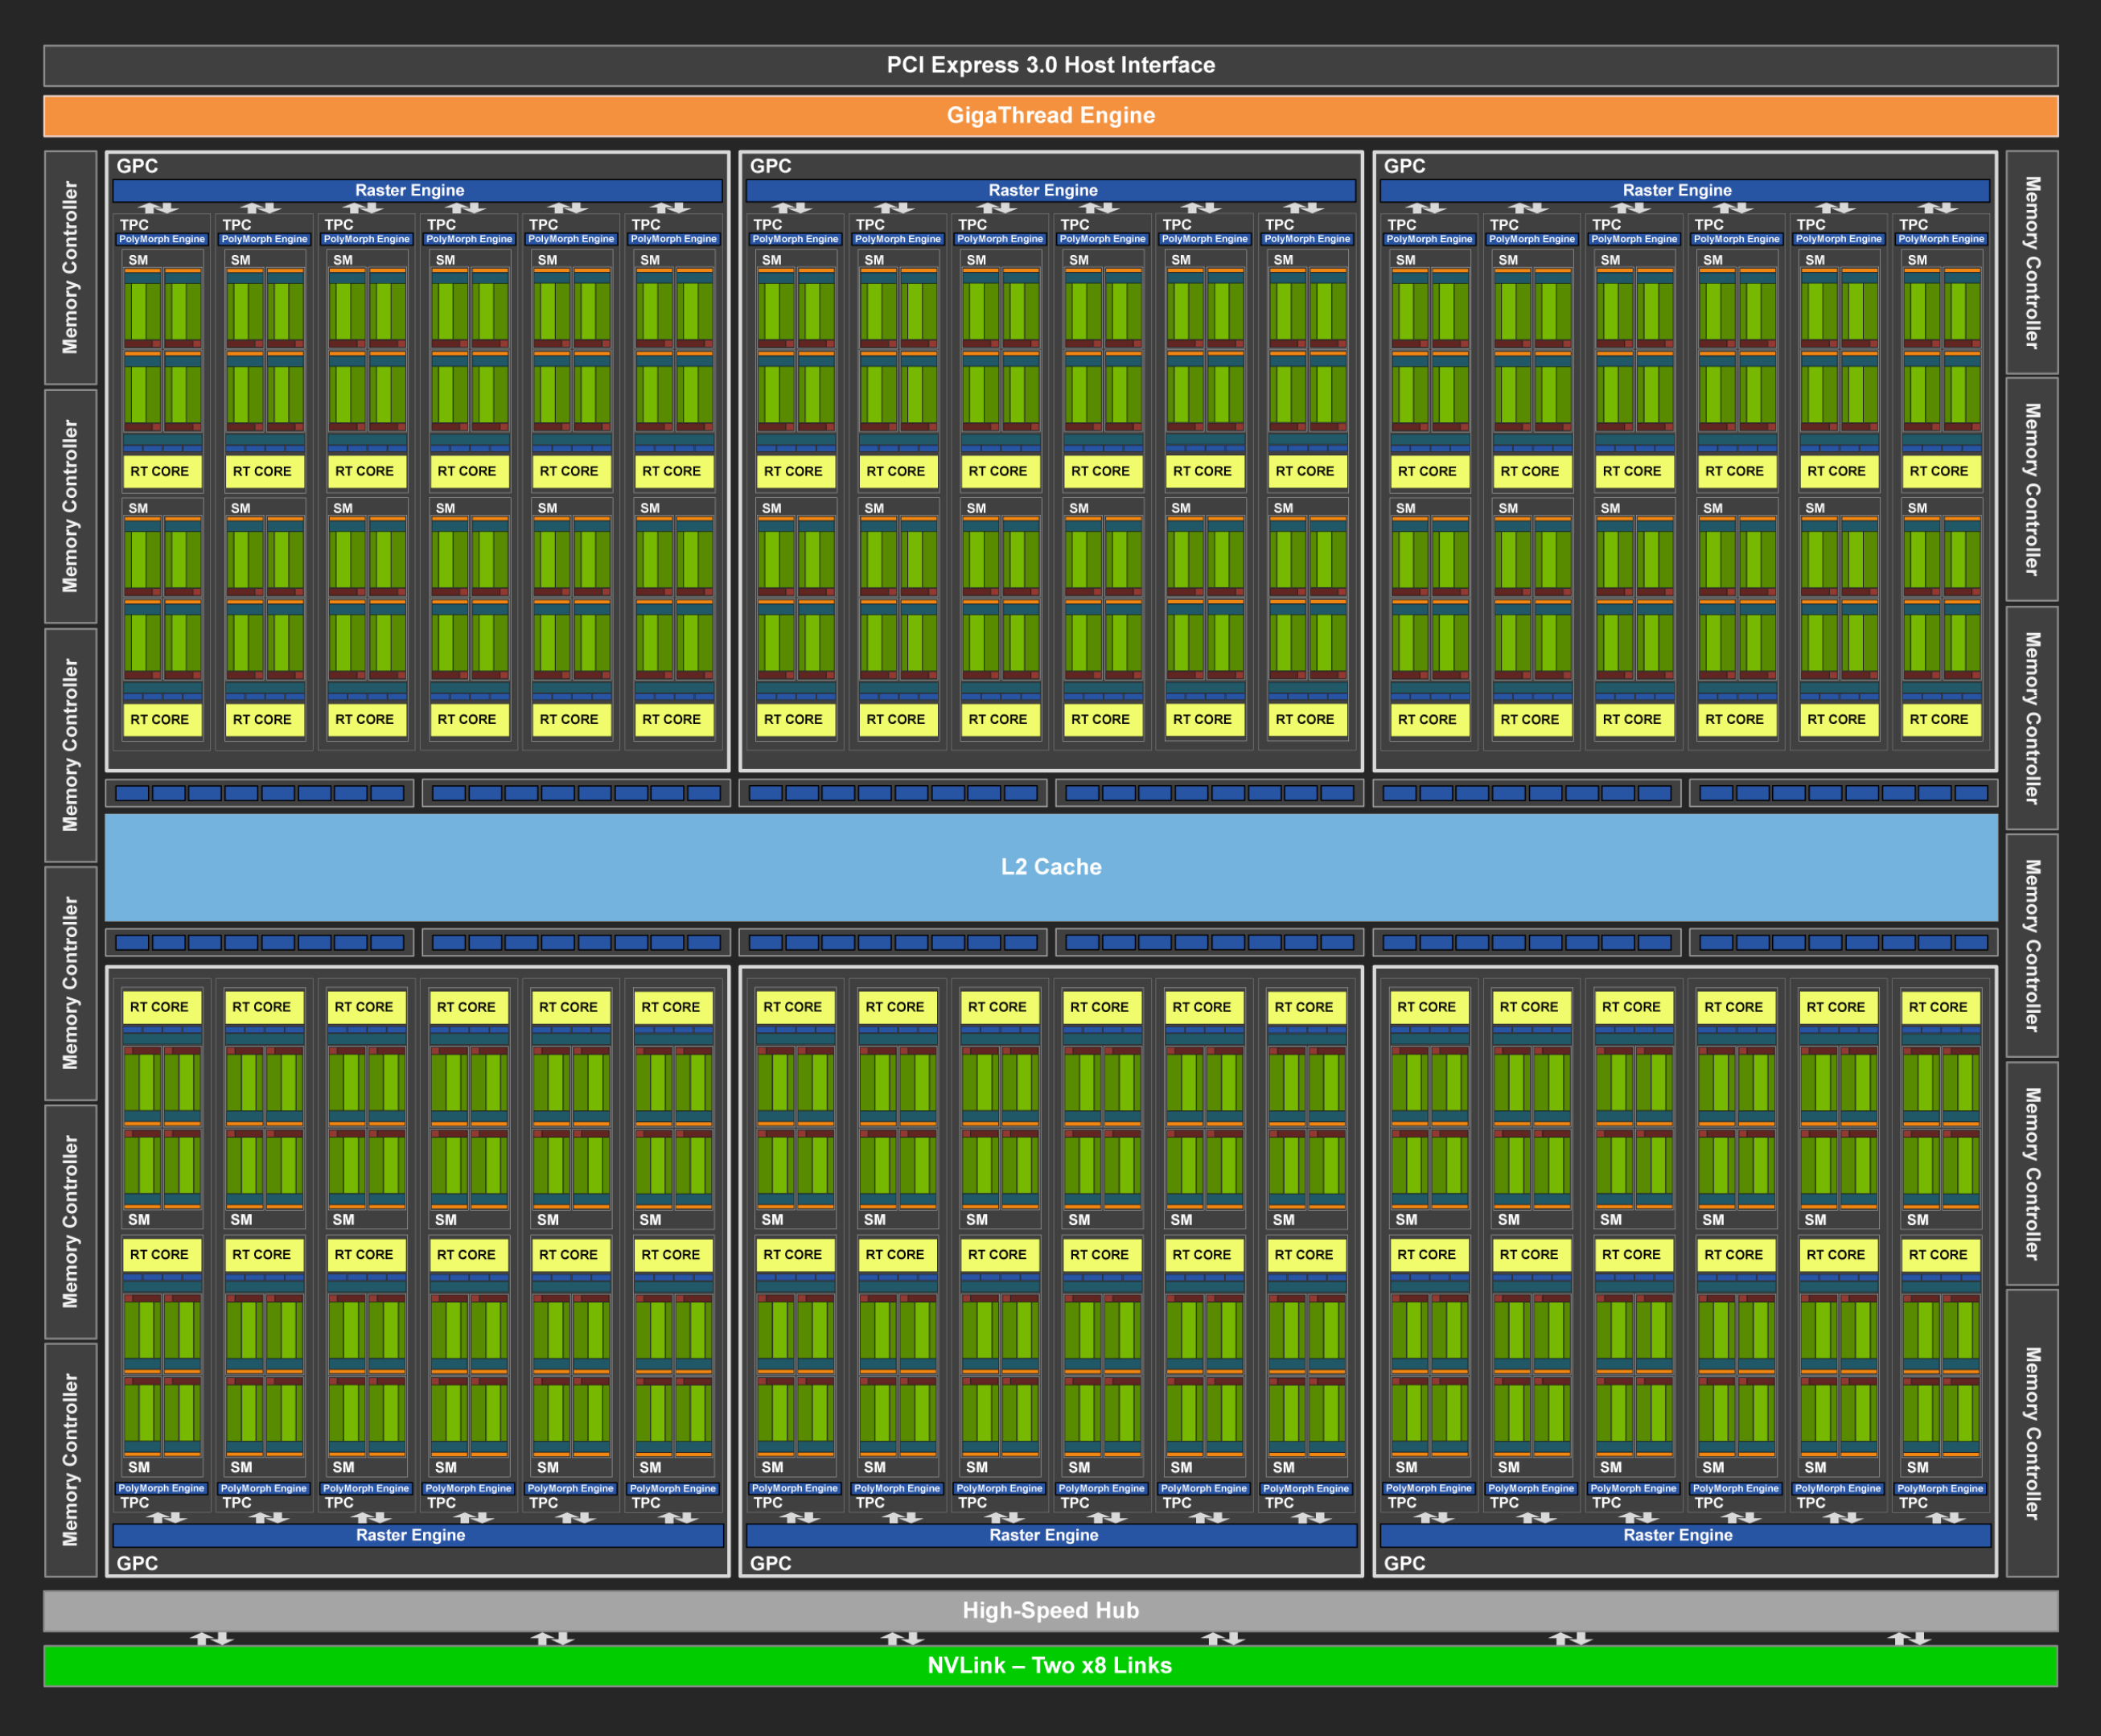
\includegraphics[width=18cm]{nvidia_turing.png}
  \centering
  \caption{Nvidia Turing架构}
  \label{fig:nvidia_turing}
\end{figure}

\begin{figure}[H]
  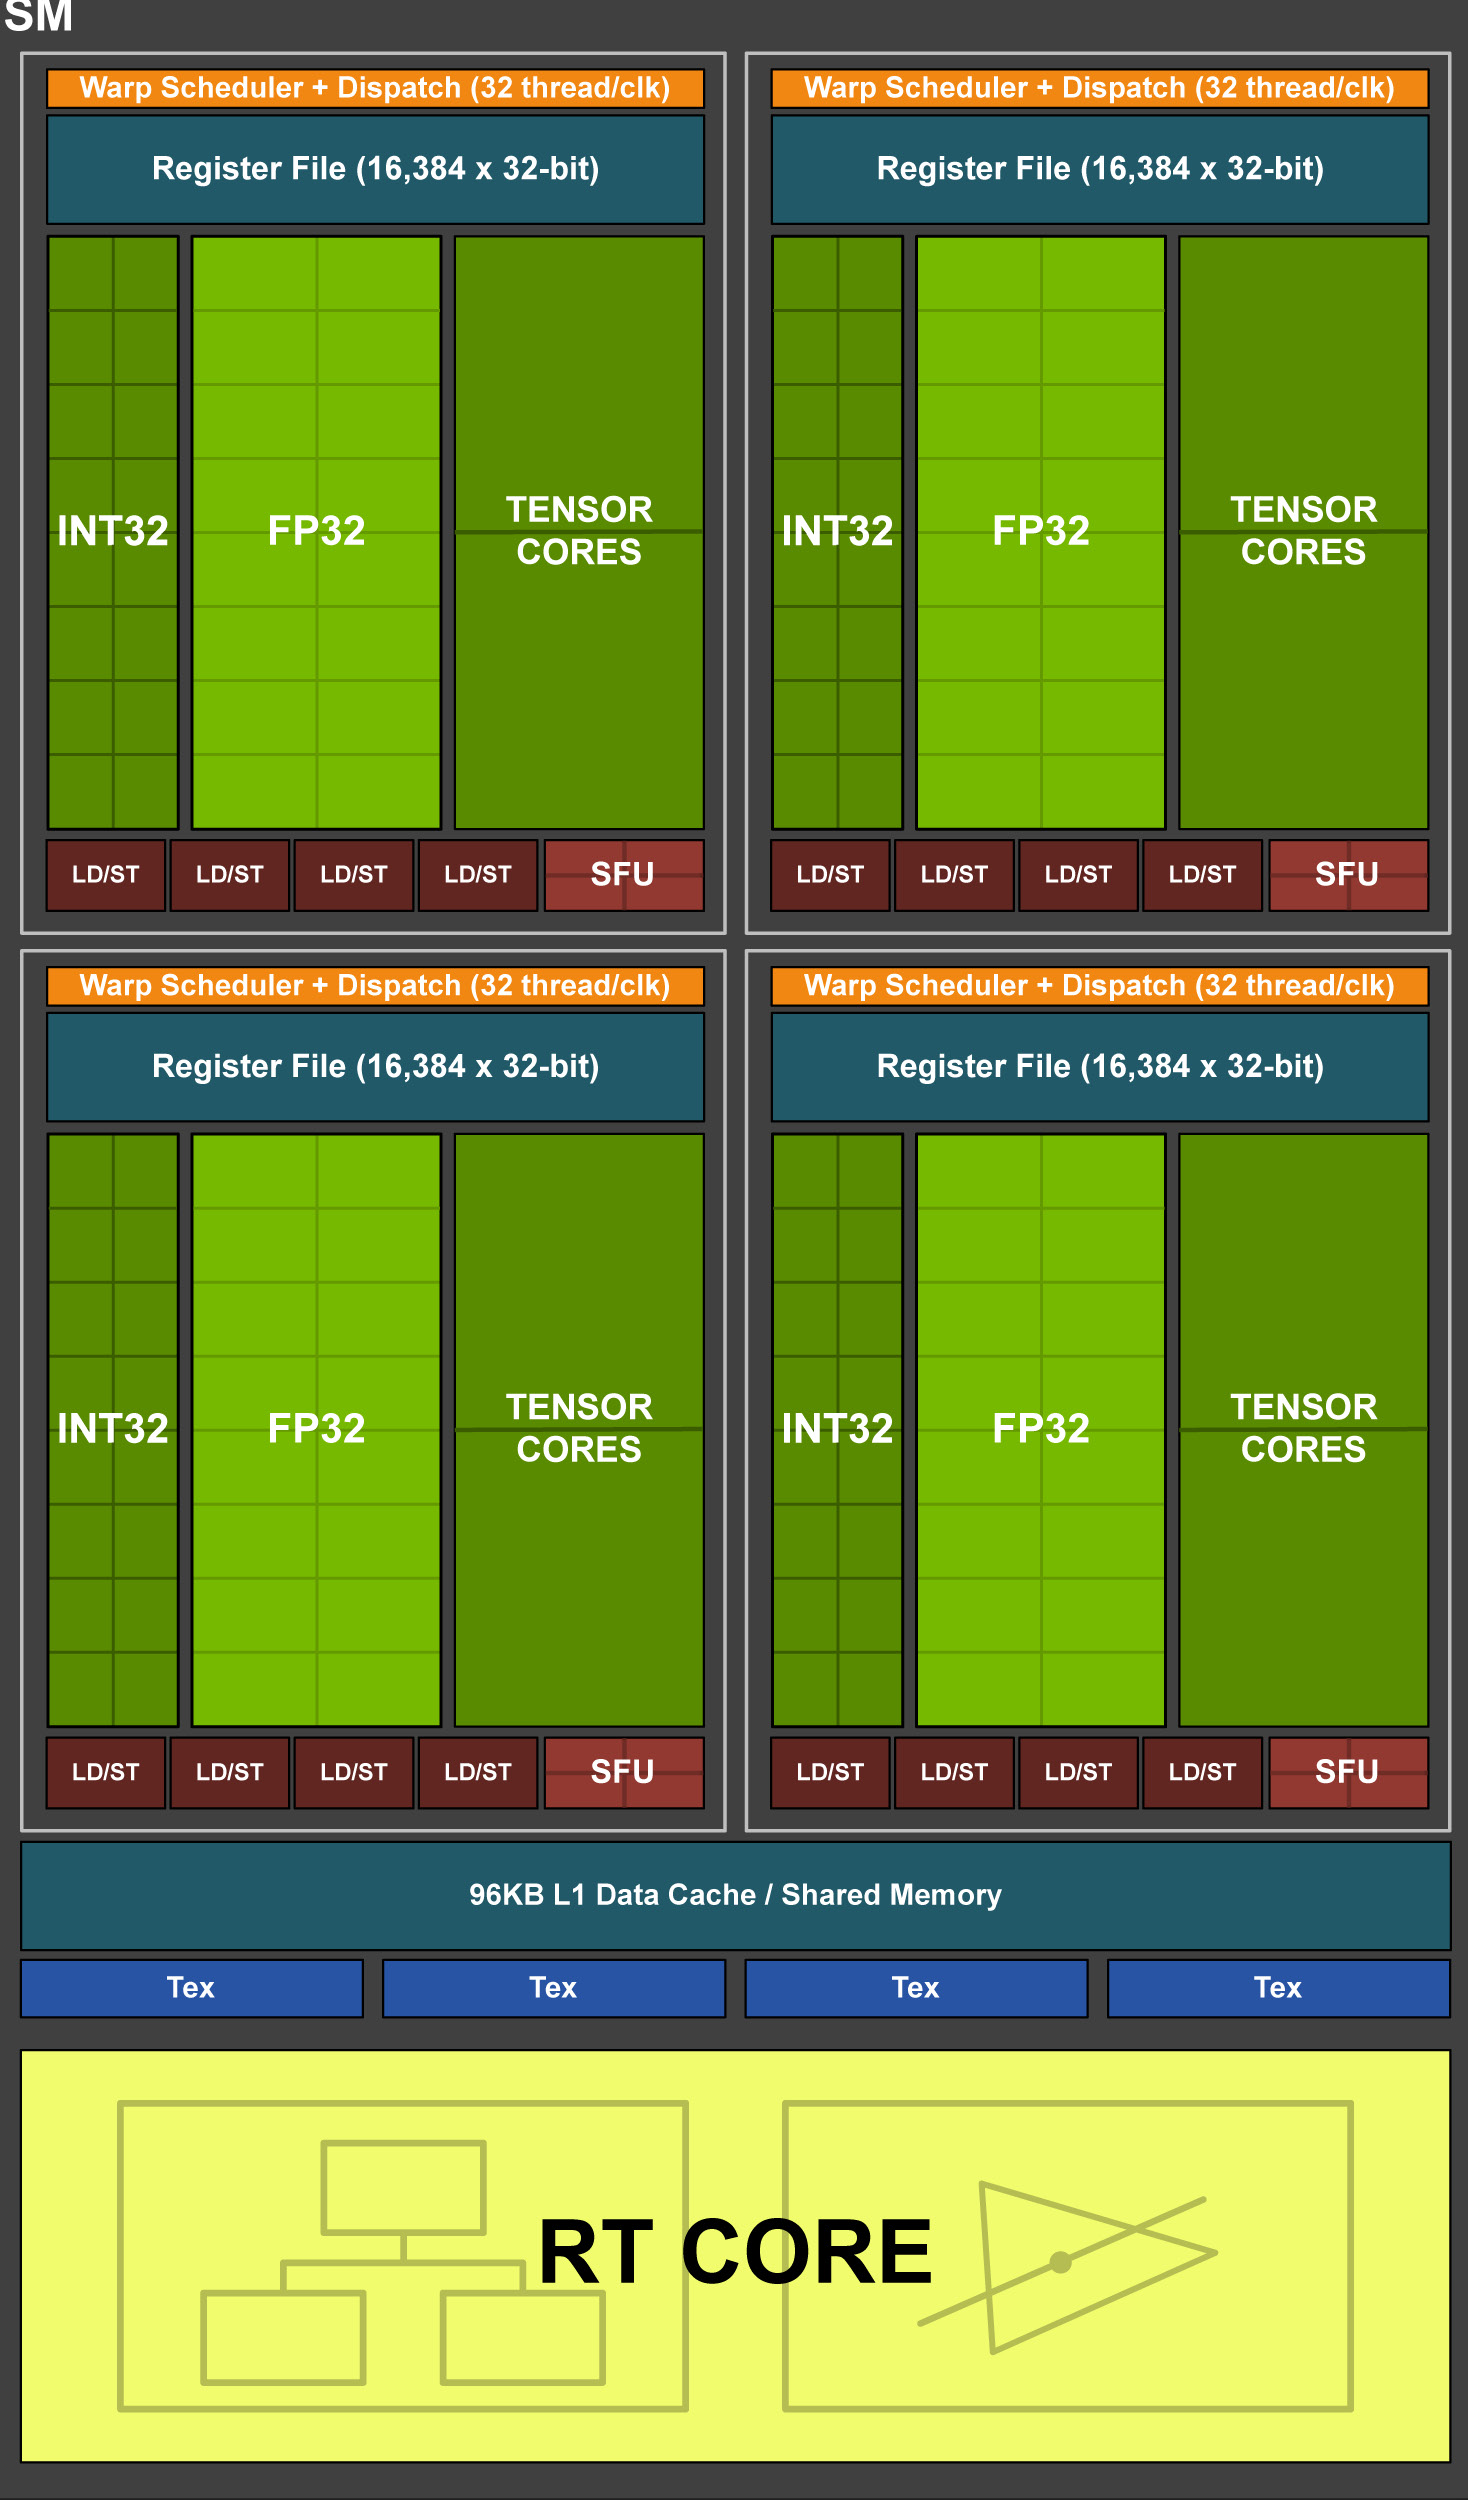
\includegraphics[width=10cm]{nvidia_turing1.png}
  \centering
  \caption{Nvidia Turing架构-Stream Multiprocessor}
  \label{fig:nvidia_turing_SM}
\end{figure}

\begin{itemize}
\item Giga Thread Engine
  管理所有正在进行的工作
\item GPC(Graphics Processing Cluster)
  \\GPU被划分成多个GPCs(Graphics Processing Cluster), 每个GPC拥有多个SM(SMX、SMM)和一个光栅化引擎(Raster Engine).
  \begin{itemize}
  \item Raster Engine
  \item TPC(Texture Processing Cluster)
    \begin{itemize}
    \item PolyMorph Engine
      \\多边形引擎负责属性装配(attribute Setup)、顶点拉取(VertexFetch)、曲面细分、栅格化
    \item Register File
    \item SM(Stream Multiprocessor)
      \\多个sp加上其他的一些资源组成一个SM, 其他资源也就是存储资源, 共享内存, 寄储器等.
    \item Warp(Warp Schedular+Dispatch)
      \\多个SP(一般是32个)组成一个Warp, Warp是最小调度单位. 同一个Warp内的SP执行指令相同只是数据不同. 只有全部线程执行完毕才会进行下一个Warp的工作.
    \item SP(Stream Processor)/Core/Thread
      \\SP是最基本的处理/计算单元.
      \begin{itemize}
      \item ALU
      \item FPU
      \item Tensor Core
      \end{itemize}
    \item SFU
      \\特殊数学函数, 如sin, cos, 与普通sin, cos实现(一般会查表)不同.
    \item L1 Cache
    \item Texture Cache
    \item LD/ST
    \item RT(RayTracying) Core
    \end{itemize}
  \end{itemize}
\item Grid
  \\编程中的一个概念. 指在GPU上由多个Thread block(SM)执行的一套代码.
\end{itemize}

\subsubsection{GPU的内存分级}
GPU内存等级(参考《Computer Architecture》\cite{hennessy_computer_nodate})
\begin{center}
  \begin{tabular}{| m{8em} | m{8em} | m{10em} | m{12em} |}
    \hline
    \textbf{More descriptive name} & \textbf{Closest old term outside of GPUs} & \textbf{Official Nvidia GPU term} & \textbf{Description} \\ [0.5ex] 
    \hline
    GPU Memory & Main Memory & Global Memory & DRAM memory accessible by all multithreaded SIMD Processors in a GPU.\\
    \hline
    Private Memory & Stack or Thread Local Storage (OS) & Local Memory & Portion of DRAM memory private to each SIMD Lane.\\
    \hline
    Local Memory & Local Memory & Shared Memory & ast local SRAM for one multithreaded SIMD Processor, unavailable to other SIMD Processors\\
    \hline
    SIMD Lane Registers & Vector Lane Registers & Thread Processor Registers & Registers in a single SIMD Lane allocated across a full thread block (body of vectorized loop).\\
    \hline
  \end{tabular}
\end{center}

访存速度:
\begin{center}
  \begin{tabular}{| m{6em} | m{6em} | m{6em} | m{6em} | m{6em} | m{8em} | m{5em} |}
    \hline
    \textbf{存储类型} & \textbf{寄存器} & \textbf{共享内存} & \textbf{L1缓存} & \textbf{L2缓存} & \textbf{纹理、常量缓存} & \textbf{全局内存}\\
    \hline
    \textbf{访存周期} & 1 & 1 -- 32 &	1 -- 32	& 32 -- 64	& 400 -- 600	& 400 -- 600\\
    \hline
  \end{tabular}
\end{center}

\subsection{GPU渲染总览}
现代GPU有着相似的结构, 有很多相同的部件, 在运行机制上, 也有很多共同点. 这里以Nvidia-Fermi架构为例:
\begin{figure}[H]
  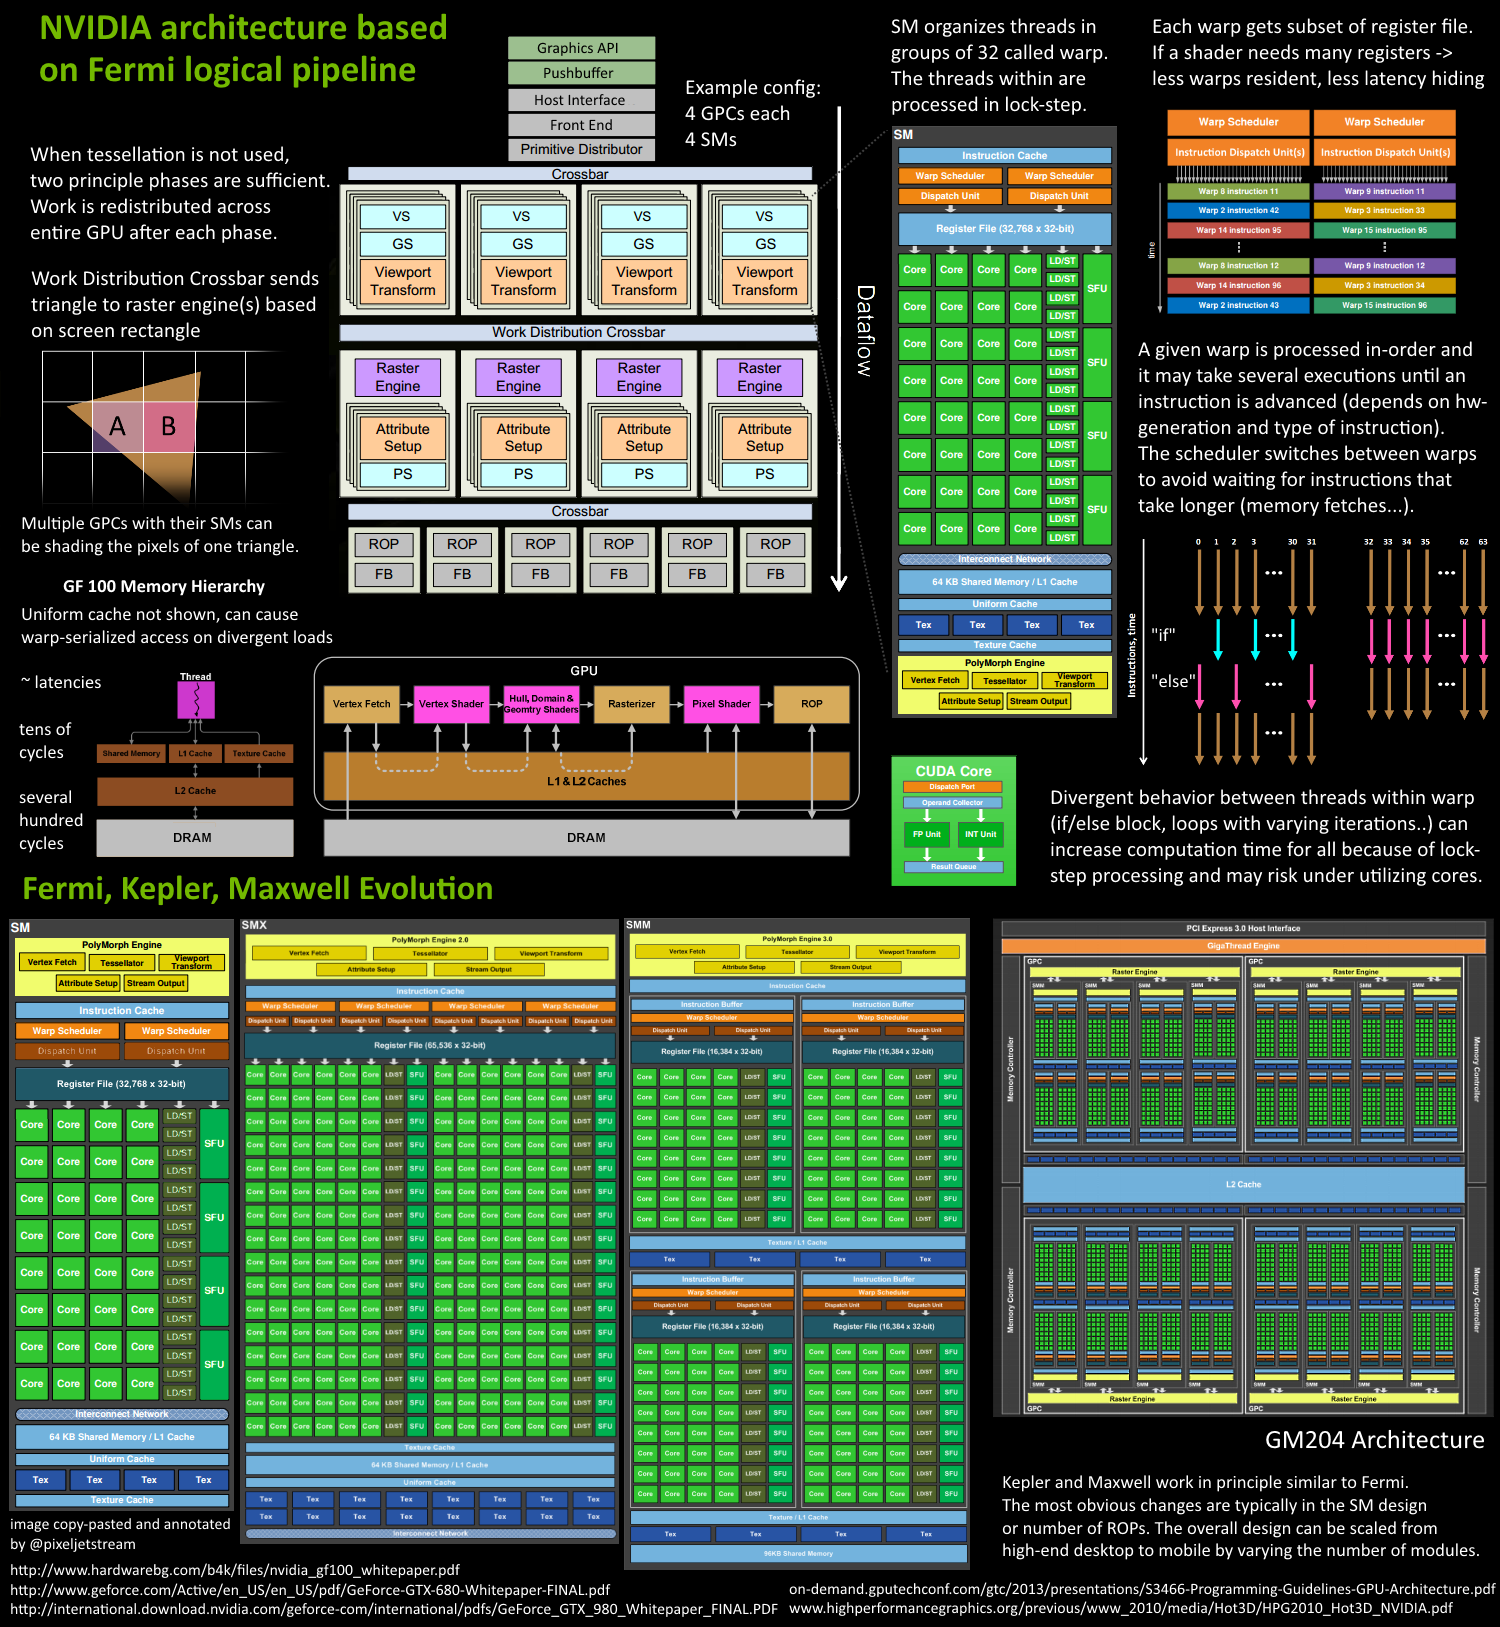
\includegraphics[width=18cm]{gpu_rendering_overview.png}
  \centering
  \caption{GPU渲染管线的执行细节}
  \label{fig:nvidia_fermi_rendering_pipeline}
\end{figure}

从Fermi开始NVIDIA使用类似的原理架构, GPU中使用Giga Thread Engine来管理所有正在进行的工作. GPU被划分为多个GPC, GPC通过Crossbar与其他功能模块相连.

程序员编写的shader是在SM上完成的. 每个SM包含许多为线程执行数学运算的Core(核心). 例如, 一个线程可以是顶点或像素着色器调用. 这些Core和其它单元由Warp Scheduler驱动, Warp Scheduler管理一组32个线程作为Warp(线程束)并将要执行的指令移交给Dispatch Units.

对于相同架构的GPU,  具体有多少个GPC, GPC有多少SM...则根据不同的显卡型号有所不同.

\subsubsection{GPU渲染管线的执行}
\begin{figure}[H]
  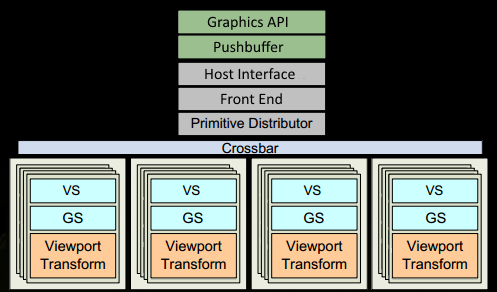
\includegraphics[width=10cm]{rendering_logic_0.png}
  \centering
  \caption{渲染管线执行: 图元数据的输入}
  \label{fig:rendering_pipeline_input}
\end{figure}

1. Drawcall $\to$ 驱动程序(合法性检查) $\to$ Pushbuffer(flush) $\to$ Host Interface(并通过Front End处理). 

2. 在图元分配器(Primitive Distributor), 将图元分成批次发送给多个PGCs.

3. 在GPC的SM中的Poly Morph Engine负责取出三角形的数据(vertex data).

4. 在获取数据之后, 在SM中以线程束(Warp)来调度, 来开始处理顶点数据. 这里SM的warp调度器会按照顺序分发指令给整个Warp, Warp中的线程锁步执行, 不激活状态下会被遮掩(be masked out). Shader中若有分支等价于所有分支全走一遍(除非Warp中所有线程均走同一分支). Warp中的指令可以被一次完成, 也可能经过多次调度, 例如通常SM中的LD/ST(加载存取)单元数量明显少于基础数学操作单元, 此时Warp调度器可能会简单地切换到另一个没有等待的Warp, 这也是GPU克服内存读取延迟的关键. 这里会产生一个矛盾, shader需要越多的寄存器, 就会给Warp留下越少的空间, 就会产生越少的Warp, 这时候在碰到内存延迟的时候就会只是等待, 而没有可以运行的Warp可以切换.

\begin{figure}[H]
  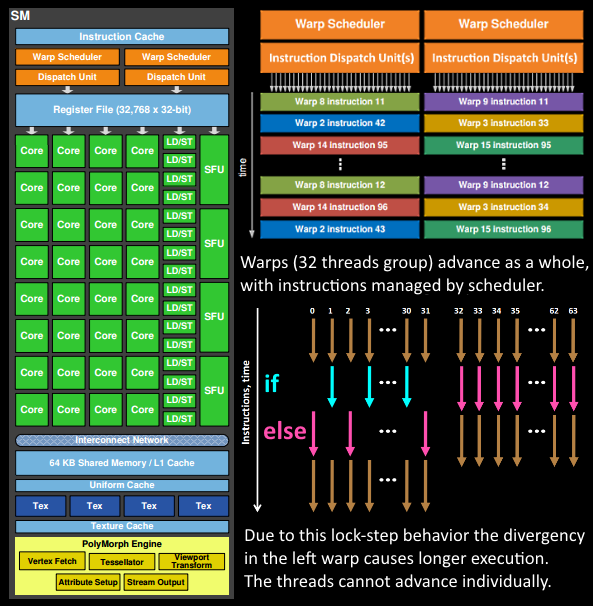
\includegraphics[width=10cm]{rendering_logic_1}
  \centering
  \caption{渲染管线执行: Execution}
  \label{fig:rendering_pipeline_shader_exec}
\end{figure}

5. Vertex Shader完成后, 运算结果会被Viewport Transform模块处理, 三角形会被裁剪然后准备栅格化, GPU会使用L1和L2缓存来进行vertex-shader和pixel-shader的数据通信.
\begin{figure}[H]
  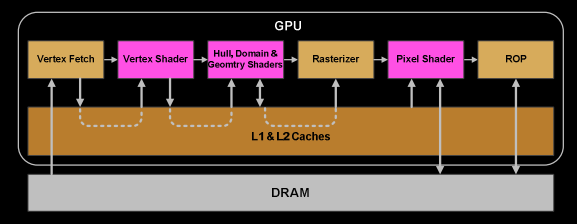
\includegraphics[width=10cm]{rendering_logic_2}
  \centering
  \caption{渲染管线执行: 各阶段完成后数据存到Cache}
  \label{fig:rendering_pipeline_stage_res}
\end{figure}

6. 接下来这些三角形将被分配给多个GPC, 三角形的范围决定着它将被分配到哪个光栅引擎(raster engines), 每个raster engines覆盖了多个屏幕上的tile, 这等于把三角形的渲染分配到多个tile上面. 也就是像素阶段就把按三角形划分变成了按显示的像素划分了.
\begin{figure}[H]
  \centering
  \subfloat[渲染管线执行: 光栅化]{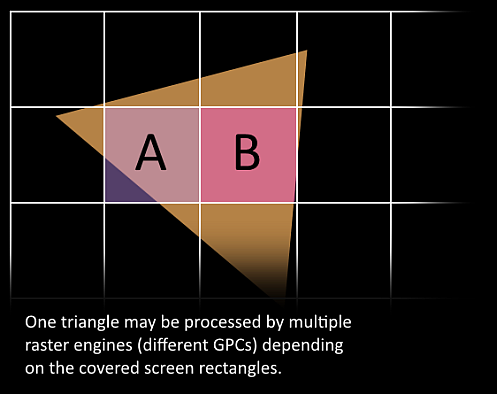
\includegraphics[width=8cm]{rendering_logic_3}}
  \subfloat[渲染管线执行: tile, Execute Pixel Shader]{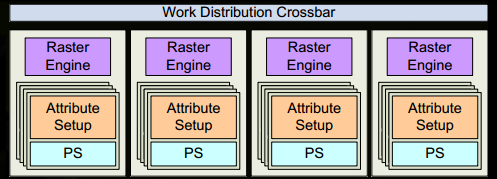
\includegraphics[width=8cm]{rendering_logic_4}}
  \caption{渲染管线执行: 光栅化+pixel shader}
  \label{fig: rendering_rastering}
\end{figure}

7. SM上的Attribute Setup保证了从vertex-shader来的数据经过插值后是pixel-shade是可读的. 

8. GPC上的光栅引擎(raster engines)在它接收到的三角形上工作, 来负责这些这些三角形的像素信息的生成(同时会处理裁剪Clipping、背面剔除和Early-Z剔除). 

9. 32个像素线程将被分成一组, 或者说8个2x2的像素块, 这是在像素着色器上面的最小工作单元, 在这个像素线程内, 如果没有被三角形覆盖就会被遮掩, SM中的warp调度器会管理像素着色器的任务. 

10. 在SM中执行Fragment/Pixel Shader.

11. 最后一步, 在ROP单元中计算深度值以及与FrameBuffer混合.

\begin{figure}[H]
  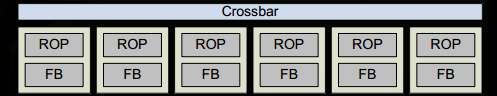
\includegraphics[width=10cm]{rendering_logic_5.png}
  \centering
  \caption{渲染管线执行: ROP进行像素点的深度值计算}
  \label{fig:rendering_pipeline_depth}
\end{figure}

\subsection{GPU技术要点}

\subsubsection{SIMD和SIMT}
SIMD(Single Instruction Multiple Data)是单指令多数据, 在GPU的ALU单元内, 一条指令可以处理多维向量(一般是4D)的数据. 比如, 有以下shader指令:
\begin{minted}{c}
  float4 c = a + b; // a, b都是float4类型
  // 对于没有SIMD的处理单元, 需要4条指令将4个float数值相加, 汇编伪代码如下:
  ADD c.x, a.x, b.x
  ADD c.y, a.y, b.y
  ADD c.z, a.z, b.z
  ADD c.w, a.w, b.w
  // 但有了SIMD技术, 只需一条指令即可处理完:
  SIMD_ADD c, a, b
\end{minted}

\begin{figure}[H]
  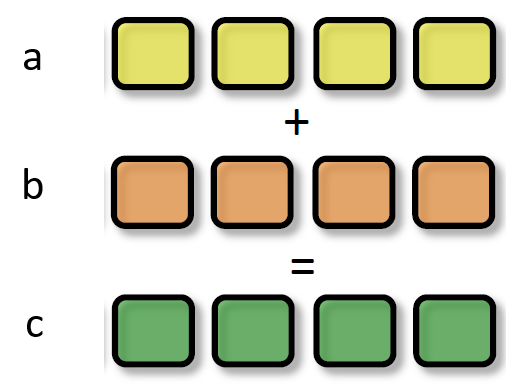
\includegraphics[width=5cm]{simd.png}
  \centering
  \caption{SIMD}
  \label{fig:simd}
\end{figure}

SIMT(Single Instruction Multiple Threads, 单指令多线程)是SIMD的升级版, 可对GPU中单个SM中的多个Core同时处理同一指令, 并且每个Core存取的数据可以是不同的.
\begin{minted}{c}
  SIMT_ADD c, a, b
\end{minted}
上述指令会被同时送入在单个SM中被编组的所有Core中, 同时执行运算, 但a、b 、c的值可以不一样:

\begin{figure}[H]
  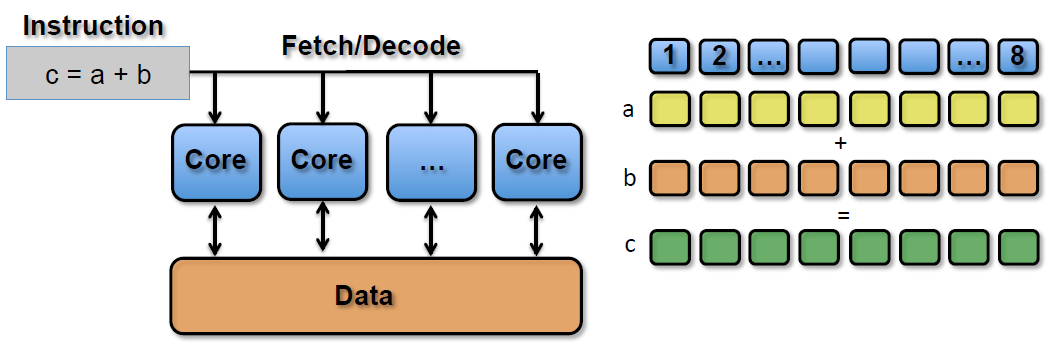
\includegraphics[width=12cm]{simt.png}
  \centering
  \caption{SIMD}
  \label{fig:simt}
\end{figure}

\subsubsection{co-issue}
co-issue是为了解决SIMD运算单元无法充分利用的问题. 为了解决着色器在低维向量的利用率低的问题, 可以通过合并1D与3D或2D与2D的指令, 提升利用率/效率.

\begin{figure}[H]
  \centering
  \subfloat[由于float数量的不同, ALU利用率从100\%依次下降为75\%、50\%、25\%]{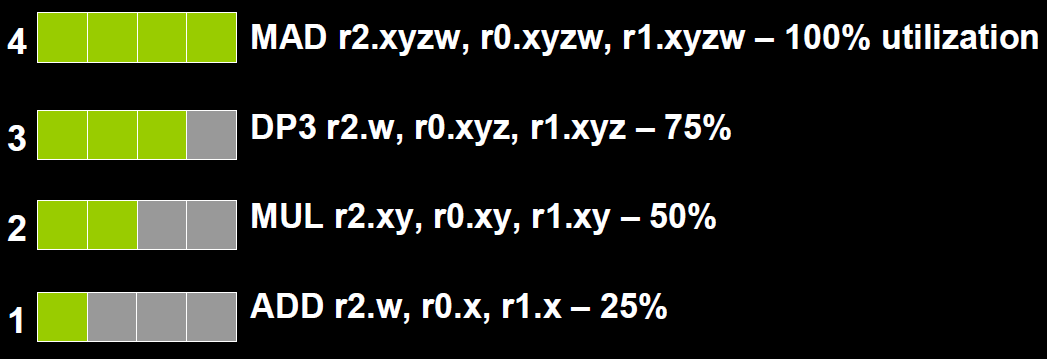
\includegraphics[width=8cm]{co-issue.png}}
  \subfloat[指令合并]{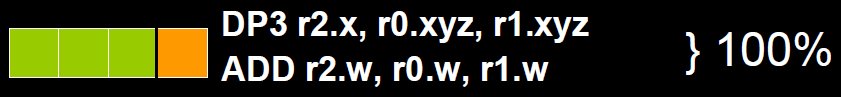
\includegraphics[width=8cm]{co-issue_1.png}}
  \caption{co-issue, 指令合并}
  \label{fig: co-issue}
\end{figure}

但是, 对于向量运算单元(Vector ALU), 如果其中一个变量既是操作数又是存储数的情况, 无法启用co-issue技术:

\begin{figure}[H]
  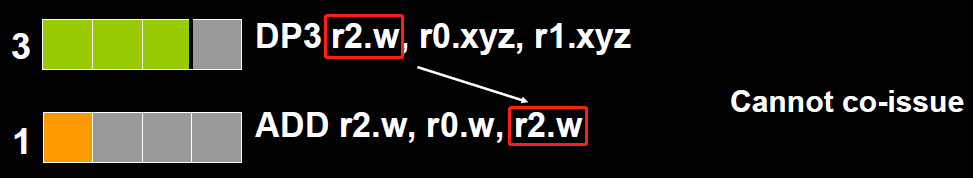
\includegraphics[width=10cm]{co-issue_2.png}
  \centering
  \caption{无法合并的情况}
  \label{fig:co-issue-unable}
\end{figure}

于是标量指令着色器(Scalar Instruction Shader)应运而生(register空间小, 低能耗), 它可以有效地组合任何向量, 开启co-issue技术, 充分发挥SIMD的优势.

\subsubsection{Early-Z}
早期GPU的渲染管线的深度测试是在像素着色器之后才执行(下图), 这样会造成很多本不可见的像素执行了耗性能的像素着色器计算。

\begin{figure}[H]
  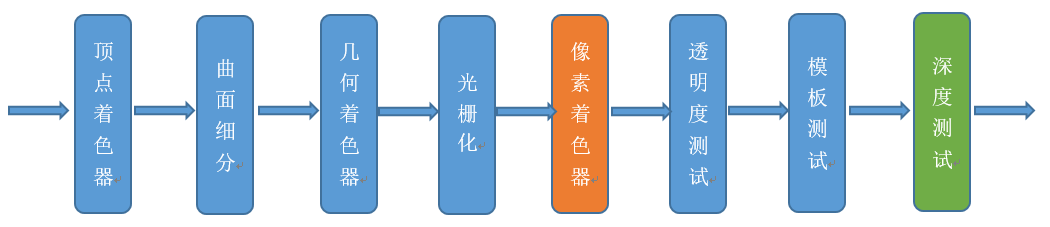
\includegraphics[width=15cm]{early_z.png}
  \centering
  \caption{早期没有Early-Z的渲染管线}
  \label{fig:rendering-pipeline-without-early-z}
\end{figure}

后来, 为了减少像素着色器的额外消耗, 将深度测试提至像素着色器之前(下图), 这就是Early-Z技术的由来.
\begin{figure}[H]
  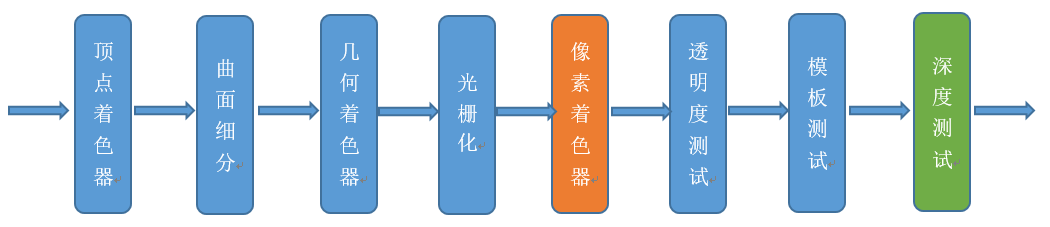
\includegraphics[width=15cm]{early_z.png}
  \centering
  \caption{添加Early-Z的渲染管线}
  \label{fig:rendering-pipeline-with-early-z}
\end{figure}

Early-Z技术可以将很多无效的像素提前剔除, 避免它们进入耗时严重的像素着色器。Early-Z剔除的最小单位不是1像素, 而是像素块(pixel quad, 2x2个像素).

  但是, 以下情况会导致Early-Z失效:
  \begin{itemize}
  \item 开启Alpha Test: 由于Alpha Test需要在像素着色器后面的Alpha Test阶段比较, 所以无法在像素着色器之前就决定该像素是否被剔除.

  \item 开启Alpha Blend: 启用了Alpha混合的像素很多需要与frame buffer做混合, 无法执行深度测试, 也就无法利用Early-Z技术.

  \item 开启Tex Kill: 即在shader代码中有像素摒弃指令(DX的discard, OpenGL的clip)。
  关闭深度测试。Early-Z是建立在深度测试看开启的条件下, 如果关闭了深度测试, 也就无法启用Early-Z技术。

  \item 开启Multi-Sampling: 多采样会影响周边像素, 而Early-Z阶段无法得知周边像素是否被裁剪, 故无法提前剔除.

  \end{itemize}

\subsubsection{统一着色器架构(Unified shader Architecture)}
在早期的GPU, 顶点着色器和像素着色器的硬件结构是独立的, 它们各有各的寄存器、运算单元等部件. 这样很多时候, 会造成顶点着色器与像素着色器之间任务的不平衡.
于是, 为了解决VS和PS之间的不平衡, 引入了统一着色器架构(Unified shader Architecture). 用了此架构的GPU, VS和PS用的都是相同的Core. 也就是, 同一个Core既可以是VS又可以是PS、GS、CS.

\subsubsection{渲染模式}

不同的渲染模对比参考\cite{render_mode_comp}:

IMR: 一种设计比较简单的流水线作业多架构方式, PC端主流. 图元数据获取后(draw call)直接渲染(走一整个流程). 阶段之间, 通过显存进行数据交互, 一帧之中会多次读写Color/Depth Buffer, 高带宽.

\begin{figure}[H]
  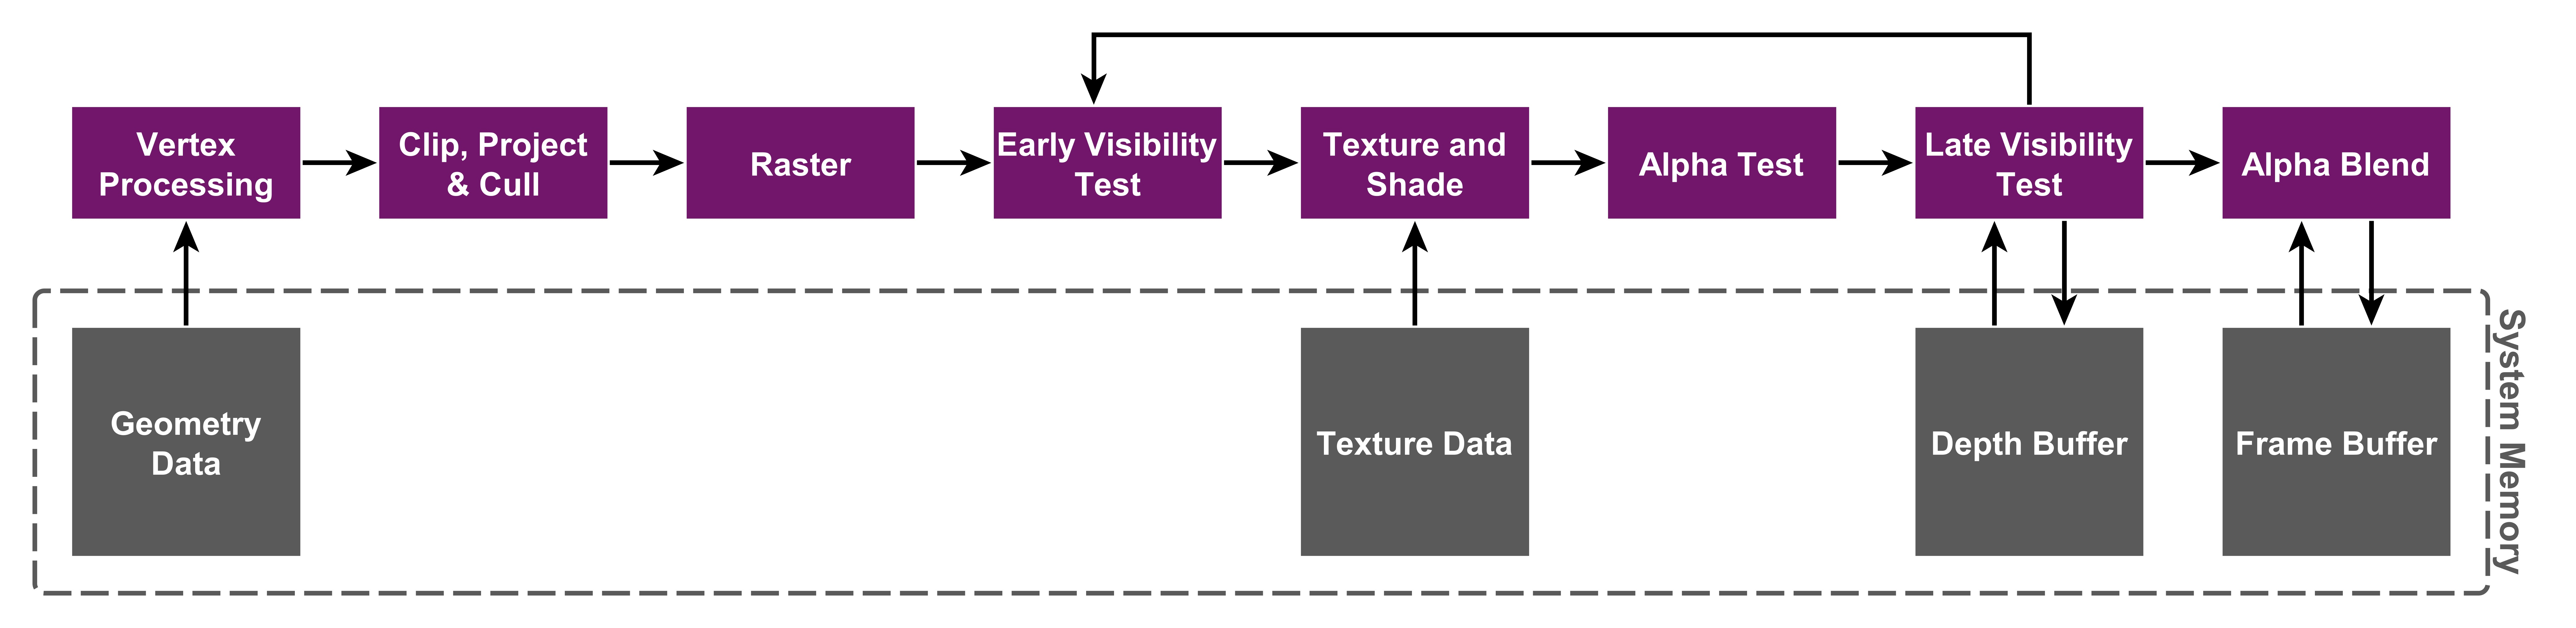
\includegraphics[width=15cm]{IMR-Pipeline-1.jpg}
  \centering
  \caption{Immediate Mode Rendering pipeline}
  \label{fig:imr}
\end{figure}

TBR: 传统移动端架构渲染模式. 通过延时渲染, 减少过度绘制. 基于Tile的渲染, 可将Color/Depth Buffer直接放在On\_Chip Memory中, 减少了主存读写. 满足移动端功耗/发热的要求.

\begin{figure}[H]
  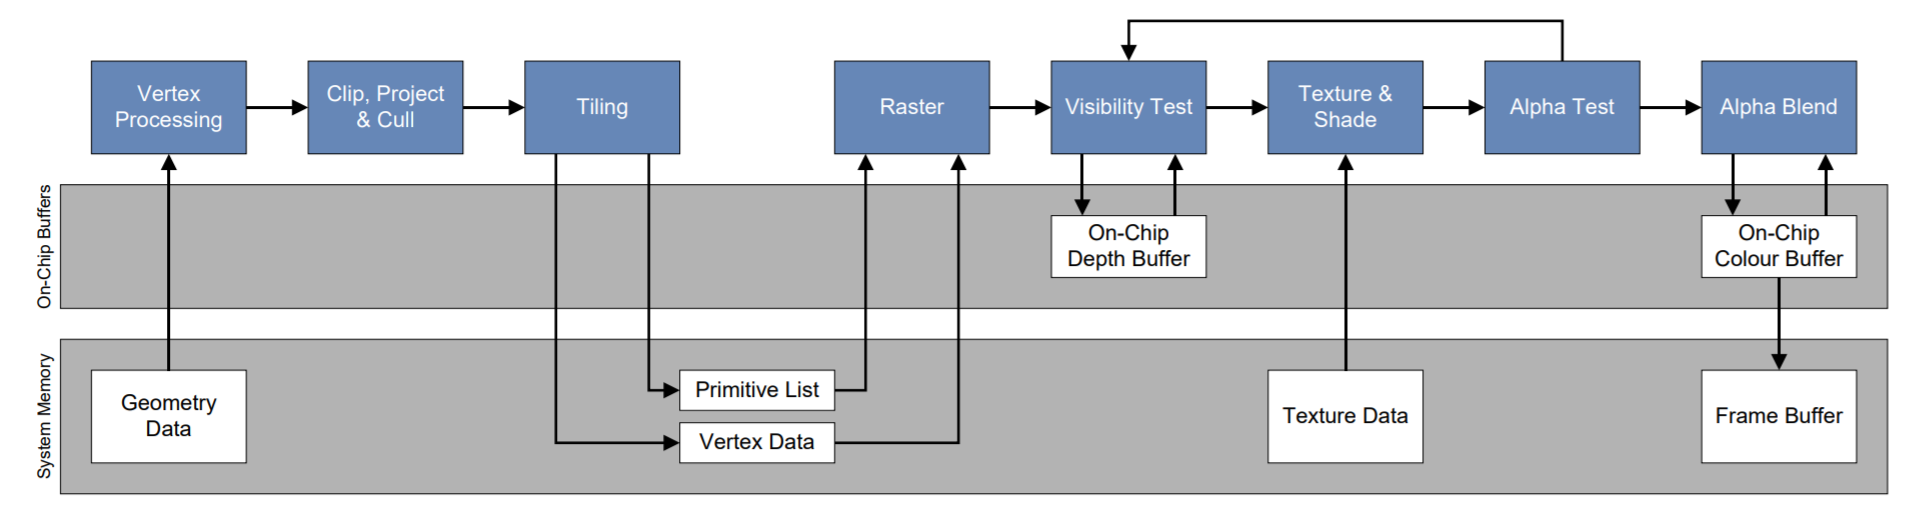
\includegraphics[width=15cm]{tbr.png}
  \centering
  \caption{Tile-Based Rendering (TBR) pipeline}
  \label{fig:tbr}
\end{figure}

理想的并行渲染, 希望GPU内部资源(SM、Raster)被充分利用, 每个硬件之间不需要通信. 但渲染过程是有顺序的, 而且在最后阶段需要统筹排序(无论深度测试还是Blend混合). IMR和TBR的不同在于, 前者在最后阶段进行排序, 简单高效. 而后者在中间阶段将Pipeline打断, 进行排序, 复杂, 但可以优化使减少无效绘制.

\vspace*{1\baselineskip}

IMR的pipeline畅通无干扰, sorting简单, TBR的sorting较复杂, 但也给低功耗优化提供了灵活的选择. 另外TBR/TBDR pipeline的分割让pipeline中断了, 各种defer, 跟IMR比起来, 速度也可能会进一步被影响而变慢.

\vspace*{1\baselineskip}

TBR用增大memory resource, 以及(有可能)降低render rate的代价, 获得降低bandwidth, power的效益.

\begin{figure}[H]
  \centering
  \subfloat[TBDR sort middle]{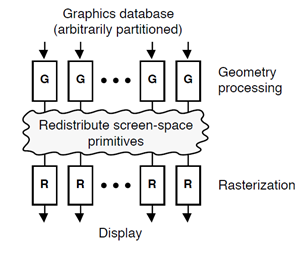
\includegraphics[width=6cm]{tbdr_sort_middle.png}}
  \subfloat[IMR sort last]{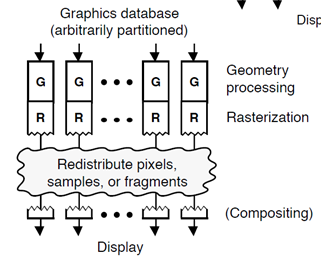
\includegraphics[width=6cm]{imr_sort_last.png}}
  \caption{TBR与IMR渲染过程上的区别\cite{render_mode_comp}}
  \label{fig: rendering_rastering}
\end{figure}

\begin{figure}[H]
  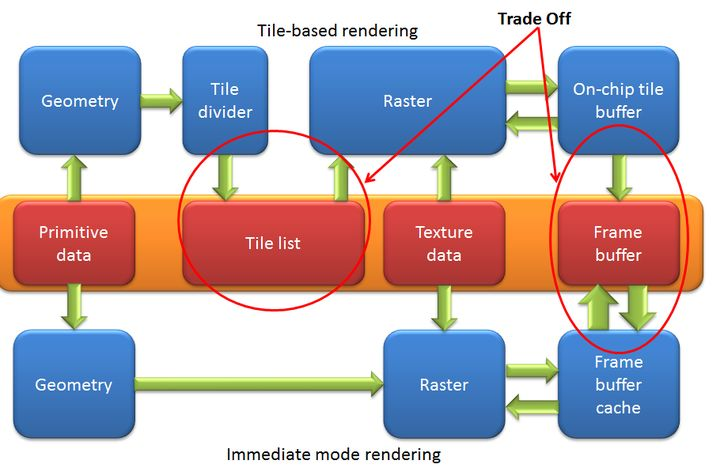
\includegraphics[width=12cm]{tbdr_imr_memory.jpg}
  \centering
  \caption{TBDR、IMR访存上的区别}
  \label{fig:tbdr}
\end{figure}


TBDR: 现代移动端渲染模式. 加入HSR, 进一步降低了过度绘制. PowerVR的专利, Apple最新的GPU也用了HSR, 应该向PowerVR交钱了.

\begin{figure}[H]
  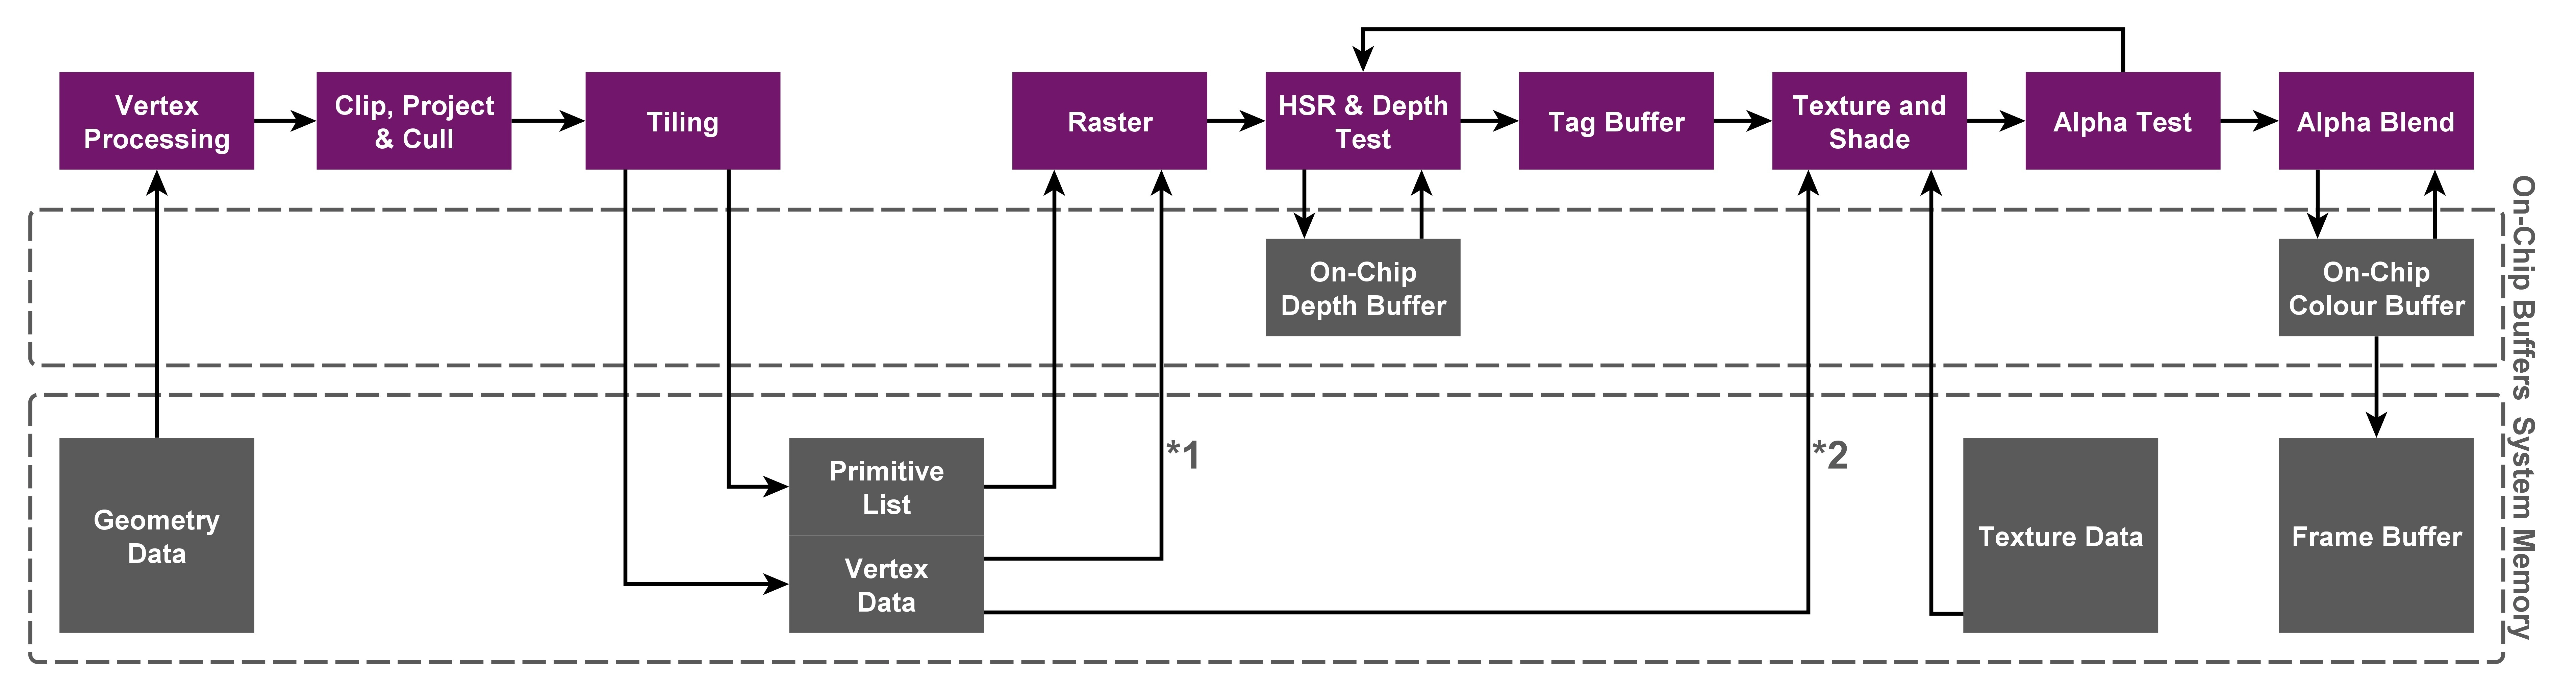
\includegraphics[width=15cm]{tbdr.png}
  \centering
  \caption{Tile-Based Deferred Rendering (TBDR) pipeline\cite{powerVR_int}}
  \label{fig:tbdr}
\end{figure}

虽然, 现代GPU有Early-Z可以剔除遮挡, 但是对与深度上的遮挡任然取决与绘制的顺序. TBDR通过再一次延迟, 让Early-Z不再依赖于绘制顺序, 最大程度上剔除无效片元. 当一个像素通过了Early-Z准备执行PS进行绘制前, 先不画, 只记录标记这个像素归哪个图元来画. 等到这个Tile上所有的图元都处理完了, 最后再真正的开始绘制每个图元中被标记上能绘制的像素点.

TBDR的渲染流程:
\begin{itemize}
\item 1. 获取图元数据, 进行Vertex Processing(Vertex Shader).
\item 2. 转换到屏幕坐标系并进行裁剪, Tiling, 划分为32$\times$32或16$\times$16的tile. 并将数据写入主存.
\item 3. 当一帧的数据集齐或强制commit/flush时, 从主存中读取数据, 进行光栅化. 然后HSR和深度测试, 丢弃不需要绘制的片元.
\item 4. 片元着色.
\item 5. Alpha测试.
\item 6. AlphaBlend.
\end{itemize}

\subsection{CPU VS GPU}
比喻:
\begin{itemize}
\item CPU 敌后特工组织. 具有强大/复杂的组织网络(CPU控制单元).  特工(核心)很强大(大Cache, 复杂指令集...), 能完成特别复杂的任务. 以任务为单位, 特工(CPU核心)数量不多, 大多时候一个特工(CPU核心)需要并发处理很多任务.
\item GPU 正面兵团. 组织结构比较简单(GPU控制单元), 具有大量的士兵(核心), 作战以小队为单位(Warp). 单个士兵能力比较简单, 适合大规模的正面作战(大数据运算).
\end{itemize}

CPUs are optimised to execute large, heavily branched tasks on a few pieces of
data at a time. \cite{powerVR_int}

GPUs are optimised to work on the principle that the same piece of code will be
executed in multiple threads, often numbering into the millions, to handle the large
screen resolutions of today’s devices. \cite{powerVR_int}

CPU - 多任务并发处理(具有强大的控制单元, Cache). GPU - 大数据并行处理(多核心, 多寄存器).
\begin{center}
  \begin{tabular}{| c  c  c |}
    \hline
     & \textbf{CPU} & \textbf{GPU} \\ [0.8ex] 
    \hline
    并行目标 & 任务(Task) & 数据(Data)\\
    \hline
    核心架构 & 多线程核心 & SIMT核心\\
    \hline
    线程数量级别 & 10 & $10^4$\\
    \hline
    吞吐量 & 低 & 高\\
    \hline
    缓存需求量 & 高 & 低\\
    \hline
    线程独立性 & 低 & 高\\
    \hline
  \end{tabular}
\end{center}

\begin{figure}[H]
  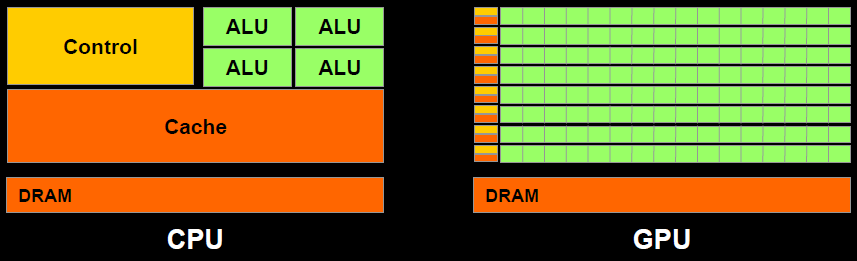
\includegraphics[width=15cm]{gpu_vs_cpu.png}
  \centering
  \caption{CPU和GPU硬件上的比较}
  \label{fig:CPU_VS_GPU}
\end{figure}

\section{渲染优化经验/建议}
参考《深入GPU硬件架构及运行机制》\cite{deepIntoGPU}
\begin{itemize}
\item 减少CPU-GPU数据交换: 合批(Batch); 减少顶点数、三角形数; 视锥裁剪(BVH, Portal, BSP, OSP); 避免每帧提交数据(CPU版的粒子, 动画每帧修改、提交数据[可移至GPU端]); 减少渲染状态的查询; 启用GPU Instance; 开启LOD; 避免从GPU读取数据.
\item 避免过度绘制: 尽可能使Early-Z有效; 开启裁剪(背面裁剪、视口裁剪、遮挡裁剪); 控制物体数量.
\item Shader代码优化: 避免if-else, switch, 可变for循环; 减少纹理采样次数; 减少复杂数学函数调用.
\end{itemize}

更多优化经验, 可参考:
\begin{itemize}
\item 《移动游戏性能优化通用技法》\cite{renderingOpt}
\item 《PowerVR Performance Recommendations The Golden Rules》\cite{powerVR_int} 或中文版本\cite{powerVR_opt_ch}
\end{itemize}
\bibliography{bibliography.bib}
\end{document}
